\documentclass[output=paper,colorlinks,citecolor=brown,arabicfont,chinesefont,booklanguage=french]{langscibook}
\ChapterDOI{10.5281/zenodo.15394491}
\author{Georgios (Yorgos) Kassiteridis\affiliation{Centre Norbert Elias – Avignon Université}}
\title[Les langues orientales dans le \emph{Dictionnaire universel} de Trévoux]
      {La valeur pragmatique des langues dites «~orientales~» dans le Dictionnaire universel de Trévoux (1721)}

\abstract{A remarkable feature of the \emph{Dictionnaire universel de Trévoux} is the increased occurrences of non-European languages therein, such as Hebrew, Arabic, and Syriac, referred to as “oriental languages” in the dictionary. A comparative study of some relevant entries illustrates that this cannot be justified by its source text, namely Basnage de Beauval's \emph{Dictionnaire universel }(1701), where these languages are not equally present. The use of “oriental languages”, particularly in the articles related to religious scriptures, leads us to associate this lexicographical innovation with the tradition of Critical Biblical Studies, represented by Louis Cappel (1585--1658) and Richard Simon (1638--1712). This interpretative approach examines the Bible in a philological-historical manner by comparing different textual versions written in various languages. This chapter aims to identify the role of the so-called “oriental languages” in the second edition of the \emph{Dictionnaire universel de Trévoux} (1721) in order to gain a better understanding of the lexicographic tools applied in the context of a controversy, as well as to capture the ideologies related to these languages in the eighteenth century.}

\IfFileExists{../localcommands.tex}{
  \addbibresource{../localbibliography.bib}
  % add all extra packages you need to load to this file

\usepackage{tabularx,multicol}
\usepackage{url}
\urlstyle{same}

\usepackage{listings}
\lstset{basicstyle=\ttfamily,tabsize=2,breaklines=true}

\usepackage{langsci-basic}
\usepackage{langsci-optional}
\usepackage{langsci-lgr}
\usepackage{langsci-osl}
% \usepackage{./langsci/styles/langsci-lgr}
% \usepackage{./langsci/styles/langsci-osl}
% \usepackage{langsci-gb4e}

\usepackage{tikz}
\usetikzlibrary{patterns,calc}
\pgfdeclarepatternformonly{south east lines}{\pgfqpoint{-0pt}{-0pt}}{\pgfqpoint{3pt}{3pt}}{\pgfqpoint{3pt}{3pt}}{
    \pgfsetlinewidth{0.6pt}
    \pgfpathmoveto{\pgfqpoint{0pt}{3pt}}
    \pgfpathlineto{\pgfqpoint{3pt}{0pt}}
    \pgfpathmoveto{\pgfqpoint{.2pt}{-.2pt}}
    \pgfpathlineto{\pgfqpoint{-.2pt}{.2pt}}
    \pgfpathmoveto{\pgfqpoint{3.2pt}{2.8pt}}
    \pgfpathlineto{\pgfqpoint{2.8pt}{3.2pt}}
    \pgfusepath{stroke}}
    
\usepackage{stmaryrd}
\usepackage{wasysym}
\usepackage{multirow}
\usepackage{caption}
\usepackage{subcaption}
\usepackage{mathrsfs}
\usepackage{qtree}

\usepackage{linguex}


  %pminos do not split footnotes
% \interfootnotelinepenalty=10000 %Footnote in Laporte chapters has to be split SN


%\DeclareIndexNameFormat{default}{%
%\nameparts{#1}%
%\usebibmacro{index:name}%
%{\index[names]}%
%{\namepartfamily}%
%{\namepartgiveni}%
% {}% L1
% {}% L2
%{\namepartprefix}% generates spurious space L3
%{\namepartsuffix}% generates spurious space L4
%}

%  {\DeclareIndexNameFormat{default}{%
%     \usebibmacro{index:name}{\index[names]}{#1}{#3}{#5}{#7}}}

%\DeclareIndexNameFormat{default}{%
%  \usebibmacro{index:name}{\sindex[nom]}{#1}{#3}{#5}{#7}}

%\DeclareIndexNameFormat{default}{%
%  \usebibmacro{index:name}{\sindex[person]}{#1}{#3}{#5}{#7}}
%\DeclareIndexNameFormat{default}{%
%\nameparts{#1} \usebibmacro{index:name}{\sindex[person]]}{\namepartfamily}{‌​\namepartgiven}{\nam‌​epartprefix}{\namepa‌​rtsuffix}}

%\newcommand{\smiley}{:)}

%\renewbibmacro*{index:name}[5]{%
%\usebibmacro{index:entry}{#1}%
%{\iffieldundef{usera}{}{\thefield{usera}\actualoperator}\mkbibindexname{#2}{#3}{#4}{#5}}}

% \newcommand{\noop}[1]{}

%remove for final
%\overfullrule=1mm

\newcommand{\tobi}[2]}}
\renewcommand{\S}[1]{\tobi{#1}{\textsc{*}}}

% this volume references
% puts: [this volume]
% already defined: \citetv
%\newcommand{\citepv}[1]{(\citeauthor{#1} \citeyear*{#1} [this volume])}
\newcommand{\citealtv}[1]{\citeauthor{#1} \citeyear*{#1} [this volume]}

%parentheses around example number
\newcommand{\pref}[1]{(\ref{#1})}

% in-text examples

\newcommand{\lnex}[1]{\textit{#1}} %target lang word
\newcommand{\lnlit}[1]{(lit.: `#1')} %literal reading
\newcommand{\lnlat}[1]{(#1)} % latinization
\newcommand{\lntrans}[1]{`#1'} %translation
\newcommand{\lnexl}[2]%
{\lnex{#1}{} \lnlat{#2}} % ex with latinization
\newcommand{\lnexlat}[3]{\lnex{#1}{} \lnlat{#2}{} \lntrans{#3}} % ex with latinization and tranl.

%ch01
\newcommand{\co}[1]{\mbox{\textbf{#1}}}

%ch09

\newcommand{\cyrbulg}[1]{\begin{otherlanguage*}{bulgarian}#1\end{otherlanguage*}}


%ch10
\newcommand{\nlp}{{\small NLP}}
\newcommand{\mwe}{{\small MWE}}
\newcommand{\rae}{{\small RAE}}
\newcommand{\lvc}{{\small LVC}}
\newcommand{\pos}{{\small P}o{\small S}}
%\newcommand{\todo}[1]{ \textcolor{red}{#1} }

%\renewcommand{\labelenumi}{\theenumi}
%\ainamefmt{{vv}{ll}{, ff}{, jj}} % fullname

\newcommand{\biberror}[1]{{\color{red}#1}}

\newcommand{\osenovaitem}{--~}
  %% hyphenation points for line breaks
%% Normally, automatic hyphenation in LaTeX is very good
%% If a word is mis-hyphenated, add it to this file
%%
%% add information to TeX file before \begin{document} with:
%% %% hyphenation points for line breaks
%% Normally, automatic hyphenation in LaTeX is very good
%% If a word is mis-hyphenated, add it to this file
%%
%% add information to TeX file before \begin{document} with:
%% %% hyphenation points for line breaks
%% Normally, automatic hyphenation in LaTeX is very good
%% If a word is mis-hyphenated, add it to this file
%%
%% add information to TeX file before \begin{document} with:
%% \include{localhyphenation}
\hyphenation{
    Beck-man
    Ngu-yen
    back-chan-nel
    back-chan-nels
    mo-not-o-nous
    ste-reo-typ-i-cal
}

\hyphenation{
    Beck-man
    Ngu-yen
    back-chan-nel
    back-chan-nels
    mo-not-o-nous
    ste-reo-typ-i-cal
}

\hyphenation{
    Beck-man
    Ngu-yen
    back-chan-nel
    back-chan-nels
    mo-not-o-nous
    ste-reo-typ-i-cal
}

  \togglepaper[12]%%chapternumber
}{}

\begin{document} 
\begin{otherlanguage}{french}
\maketitle

Une particularité marquante du \emph{Dictionnaire universel de Trévoux} est son identité bilingue (français-latin) ainsi que l'amplification de ses pratiques plurilingues au fur et à mesure de différentes éditions qui s’échelonnent sur tout le XVIIIe siècle (de 1704 à 1771). L’usage du latin\footnote{Il s’agit d’une innovation, puisque les rédacteurs du \emph{Dictionnaire universel de Trévoux} reprennent une pratique déjà ancienne (à l'instar notamment de Robert Estienne et de Jean Nicot), alors que la généalogie sur laquelle ils se fondent, celle de Furetière (puis Basnage de Beauval) et des dictionnaires de langue comme celui de Richelet ou de l'Académie française, avait produit des dictionnaires monolingues.} et des langues européennes est analysé par Chantal \citet{Wionet1998,Wionet2006}. On constate également la présence accrue de langues non européennes telles que l’hébreu, l’arabe, le syriaque, désignées dans l’édition trévoltienne, comme nous le verrons plus loin, comme «~langues orientales~». Cet intérêt ne peut pas se justifier par rapport à son texte source, à savoir le \emph{Dictionnaire universel} (1701) de Basnage de Beauval, où ces langues ne sont pas présentes de manière égale, ni même encore précédemment à celui de \citet{Furetière1690}. Le recours aux langues orientales, particulièrement dans les articles relatifs aux écritures religieuses, nous amène à lier cette innovation lexicographique aux études bibliques critiques \citep{Laplanche1994}, comme les travaux de Louis Cappel (1585--1658) et de Richard Simon (1638--1712), qui abordent l'interprétation de la Bible de manière philologico-historique à travers la mise en regard des versions et des langues. La présente étude vise ainsi à approfondir et à identifier les rôles et les finalités des langues orientales dans le \emph{Dictionnaire universel de Trévoux} (1721), afin d’enrichir notre compréhension des outils lexicographiques appliqués dans le contexte d’une controverse de nature religieuse et commerciale, ainsi que pour percevoir les imaginaires linguistiques des langues orientales au XVIIIe siècle.

Pour ce faire, mon analyse se fonde sur un échantillon d’entrées tirées des lettres A et D de la deuxième édition du \emph{Dictionnaire universel de Trévoux} publié par l’imprimerie de Trévoux en 1721, édition anonyme (comme la première) supervisée par Etienne Souciet (1671--1744), bibliothécaire au collège jésuite Louis-le-Grand (\emph{Mémoires de Trévoux}, avril 1744~: 753). Le choix de cette édition n'est pas arbitraire~; il s’agit d’une édition qui s’écarte davantage de ses origines (du \emph{Dictionnaire universel} de Basnage de Beauval et celui de Furetière) par rapport à son édition antérieure, ce qui illustre l’augmentation de nouvelles entrées surtout dans le domaine religieux, mais aussi géographique, onomastique, botanique \citep[137]{Leca-tsiomis2023}. Dans une première phase, j’ai recueilli, par une lecture rapprochée du dictionnaire, les entrées où s’affiche la structure «~langues orientales~», afin de comprendre quelles sont les langues concrètes qui appartiennent à ce groupe, selon les rédacteurs du Trévoux, à partir des caractéristiques linguistiques reliées aux langues orientales. Puis, j’ai utilisé cette liste de langues comme mots-clés pour identifier les entrées pertinentes et constituer le corpus de recherche.

Il faut souligner que pour l’identification des langues appartenant aux langues dites «~orientales~», je me suis d’abord focalisé sur le terme «~langues orientales~» en excluant les mentions aux peuples «~orientaux~» et leurs langues, contrairement à l'approche que j’ai suivie pour les langues individuelles (voir ci-dessous), puisque le terme «~orientaux~» pour les rédacteurs du Trévoux comprend plusieurs peuples, comme les chinois, les japonais, les arméniens, dont les langues ne partagent pas les mêmes caractéristiques linguistiques que celles attribuées aux langues orientales\footnote{«~c’est le nom qu’on donne aux Prêtres Orientaux, particulierement à la Chine et au Japon~» dans BONZE~; «~car les Arméniens \& les autres Orientaux [...] »  dans ARMÉNIEN.}. Pour illustrer cela, il suffit de consulter la sous-entrée ORIENTAL\footnote{Les références en majuscules renvoient à des entrées du \emph{Dictionnaire universel de Trévoux} (1721).} ou les langues citées comme exemples sont « l’Hébreu, le Chaldéen, le Syriaque, l’Arabe, le Copt » .

Avant même la publication de la première édition du \emph{Dictionnaire universel de Trévoux} (1704), on perçoit quelques traces d’expression d’intentions dans les huit échanges que les collaborateurs et partisans du \emph{Dictionnaire universel} de Basnage de Beauval (à savoir Basnage de Beauval, Gédéon Huet, Jean Le Clerc) ont eus avec leurs critiques trévoltiens dans les pages des \emph{Mémoires de Trévoux} (janvier-février 1701~; mars 1701~; septembre-octobre 1701), de sa contrefaçon à Amsterdam publiée chez Jean-Louis de Lorme  (mai-juin 1701~; juillet-août 170) et du \emph{Journal des sçavans} (juillet 1701). On y trouve notamment des critiques assez élaborées sur des éléments des langues hébraïque (ALEPH), arabe (ACCENT), syriaque (AB-BOT), à savoir de fautes qui viennent de l’ignorance des langues Orientales  (dans \emph{Mémoires de Trévoux}, mars 1701~: 104)\footnote{Nous y trouvons également une compréhension du rôle des langues non indoeuropéennes dans les écritures sacrées, voir «~Pour parler exactement il faut dire que les Apôtres \& les Evangelistes ont conservé dans leurs écrits de certains mots Syriaques~», dans les \emph{Mémoires de Trévoux}, mars 1701~: 109,  et une attention à la grammaire et à sa relation avec la traduction, voir «~car ces articles changent souvent, le sens du discours, \& si l’on n’en sçait la force, on ne peut pas traduire exactement les Livres sacrez en nôtre langue~» dans \emph{Mémoires de Trévoux}, mars 1701~: 107~; ce qui oriente notre hypothèse sur la relation entre l’intérêt pour les langues orientales et l’interprétation/traduction des Écritures.}. 

Par ailleurs, la comparaison entre le \emph{Dictionnaire universel} (1701) de Basnage de Beauval et celui de Trévoux 1721 illustre une multiplication de références aux langues orientales (et en plus la transcription dans une écriture non latine) dans le \emph{Dictionnaire universel de Trévoux}. En particulier, dans le corpus d’entrées comportant des références aux langues orientales concrètes (nous voyons ci-dessous les langues concernées), tirées de la lettre A de la deuxième édition du Trévoux (dorénavant sous-corpus A), 53~\% n’existe pas au niveau d’entrées dans le \emph{Dictionnaire universel} de Basnage de Beauval et seulement 29~\% de celles qui y existent comporte déjà des références aux langues orientales, sous la forme de langues individuelles (par exemple, l'arabe ou  l'hébreu). La majorité des références aux langues orientales représente donc une innovation du \emph{Dictionnaire universel de Trévoux} par rapport à sa source. En outre, dans le dictionnaire trévoltien lui-même, les rédacteurs admettent que plusieurs mots religieux proviennent de langues étrangères\footnote{«~mais même dans aucun autre Livre, à sçavoir une explication très-curieuse \& très-nette de toutes les sectes différentes en fait de Religion. Comme ces mots transferez d'une Langue étrangere dans la nostre, en font maintenant une partie, on n'a pû s'empêcher de les mettre en leur place ~» dans la Préface du \emph{Dictionnaire universel de Trévoux} (1721).}, comme l’hébreu, «~langue […] dans laquelle sont écrits la plupart des livres de l’ancien Testament qu’un bon Interprète de l’Ecriture doit savoir ~» (dans HÉBREU), et ils soulignent que «~le rapport qu'ils ont aux Langues étrangeres dont ils sont dérivez, […] sont essentielles, \& d'un très-grand secours pour les entendre ~» (Préface). L’addition de langues et d'entrées, l'intérêt déjà manifesté dans les critiques du dictionnaire de Basnage de Beauval pour les langues orientales, ainsi que l'importance de l'hébreu pour la compréhension des mots religieux - sujet pertinent pour la controverse d’où est issu ce dictionnaire - me semble bien indiquer que la présence des langues orientales dans le Trévoux n'est pas accidentelle, mais un choix conscient dont je me propose ici de saisir la logique.

Tout d’abord, pour éviter d’imposer des taxonomies contemporaines, j’ai créé une liste de caractéristiques de langues orientales à partir du contexte textuel du syntagme «~langues orientales~» dans le sous-corpus A (voir Annexe). Ensuite, un processus d'élimination a été effectué afin de comprendre ce que les rédacteurs du Trévoux désignent comme «~langues orientales~». On trouve, notamment, que l’augment syllabique «~pourroit être appliqué à la Grammaire des langues Orientales~» (dans AUGMENT). L’augment syllabique existe dans de nombreuses langues, comme le grec, le sanskrit, l'arménien, l'hébreu, les langues bantoues, etc. Mais on lit également que les langues orientales «~n’éxprimoient point les voyelles ~» (dans ASPIRATION). Un exemple hors sous-corpus A et D~: dans CONSONE, les rédacteurs du Trévoux indiquent que les Grammairiens Hébreux «~ont été imitez […] par les Grammairiens des autres langues orientales ~», un «~autres~» qui me parait être une preuve que l’hébreu appartient, pour nos rédacteurs, aux langues orientales~; ou également dans AIN, qui renvoie à une lettre de «~toutes les langues orientales ~» et qui est signalée comme «~Terme de Grammaire Hébraïque \& Arabe~». Ces deux langues nous offrent, ainsi, une porte d’entrée pour commencer à examiner l’identité des langues orientales dans le \emph{Dictionnaire universel de Trévoux}. On reconnaît aussi le syriaque et le chaldéen comme les «~filles de l’hébreu ~» (dans AMEN). Il existe d’autres langues qui pourraient être pertinentes dans une analyse qui porterait dans un corpus plus étendu, comme le phénicien, le samaritain ou l’assyrien, mais puisque leur présence dans la lettre A et D n’est pas assez fréquente pour en tirer des hypothèses soutenues, nous insistons sur les quatre langues mentionnées ci-dessus~: l’hébreu, l’arabe, le syriaque, le chaldéen. 

Si on s’éloigne pour un moment du texte dictionnairique, afin de vérifier cette idée aussi à l’aide des ressources externes, on trouve que l’hypothèse selon laquelle l’hébreu, l’arabe, le chaldéen et le syriaque se cachent derrière l’expression «~langues orientales~» s’aligne sur l’analyse de \citet{Stolzenberg2015}. En particulier, Stolzenberg a entrepris de déterminer le sujet linguistique de la philologia orientalis pendant la période entre 1650 et 1750 à partir des titres d’ouvrages publiés dans cette période. Pour y parvenir, à partir de la base bibliographique de l’OCLC WorldCat, il a tracé les titres qui contenaient des termes relatifs aux langues orientales comme «~linguae orientales~», «~philologie orientale~», «~livres orientaux~», «~érudition orientale~», «~auteurs orientaux~» et «~antiquités orientales~». Il a ainsi illustré que la philologia orientalis coïncidait avec la philologia sacra, à savoir une philologie des langues du christianisme ancien et des Écritures~– un élément que les rédacteurs du \emph{Dictionnaire universel de Trévoux} n’ignorent pas, comme on le verra ci-dessous. Notamment, Stolzenberg a constaté que les ouvrages qui font référence aux langues orientales sont relatifs à l’arabe (23 titres), l’hébreu (22 titres), le chaldéen (22), le syriaque (22 titres), l’éthiopien (10 titres), le persan (10 titres), le samaritain (9 titres), le turc (6 titres), l’arménien (3 titres), le copte (3 titres), le rabbinique/hébreu mishnaïque (2 titres), le phénicien (1 titre), le grec (1 titre). Les quatre langues les plus fréquentes correspondent à l’hypothèse de cette étude.

À partir de ces entités linguistiques, j’ai identifié des mots-clés pour ancrer la lecture conséquente afin de retrouver les entrées concernées~; ces mots-clés sont soit le nom de la langue au masculin, soit la langue comme adjectif au féminin pour désigner la langue, soit les noms du peuple associé~: «~hébreu~» /(langue) «~hébraïque~» / (les) «~Juifs~» (appellent/nomment)/ «~Hébreux~», «~arabe~» / «~Arabes~», «~syriaque~» / «~Syriens~», «~chaldéen~»  / «~chaldaïque~» / «~Chaldéens~». En parcourant les lettres A et D du \emph{Dictionnaire universel de Trévoux}, j’ai composé une liste d’entrées dictionnairiques où apparaissent ces mots-clés en leur associant des métadonnées comme (i) le domaine de l’entrée, (ii) l’orientation religieuse\footnote{Puisque parfois le domaine d’une entrée est marqué comme «~nom propre~», mais on découvre que le nom se réfère à un personnage des Écritures (par exemple ABIBON).}, (iii) la présence d’une entrée du Trévoux dans le \emph{Dictionnaire universel} de Basnage de Beauval et (iv) l’existence de langues orientales aux entrées de ce dernier. Lorsque le domaine est explicitement indiqué dans l’entrée dictionnairique, il est conservé dans les métadonnées~; lorsque cette information est absente, un domaine général est déduit du contexte. Cette pratique permet une première orientation, mais risque d’imposer des éléments extérieurs au corpus. Cela exige donc la vérification des hypothèses qui s’appuient sur ces domaines avec d’autres métadonnées. Quant à l’orientation religieuse d’une entrée (voir «~sujet religieux~»), la classification est basée sur les références explicites à des livres d’Écritures saintes (voir Genèse, Livres des Rois) ou à des œuvres de la tradition catholique telles que celles consacrées aux saints de l’Église catholique (Acta Sanctorum)\footnote{Si la référence à ces œuvres est liée à un exemple d’usage du terme sans commentaires (comme source d’un exemple), l’entrée n’est pas considérée comme référant à un sujet religieux.}. Les entrées sur les sectes et l’histoire comparée des religions, lorsqu’elles ne comportent pas de références explicites aux œuvres mentionnées, ne sont pas prises en considération pour cette étude pour la catégorie «~sujet religieux~», car elles présentent également un intérêt pour les informations ethnographiques et pas seulement pour les études bibliques critiques, intérêt qui nécessiterait une étude dédiée pour l’approfondir. La classification de langues suit la même méthode en se concentrant sur les références explicites des langues et la présence de mots dans une langue orientale dans l’entrée. Dans le cas où la langue n’est pas indiquée par les rédacteurs, la langue est classifiée comme «~non spécifiée~». De surcroît, la comparaison avec le \emph{Dictionnaire universel} de Basnage de Beauval est effectuée au niveau d’entrées et de sous-entrées~; en particulier, j’ai cherché à savoir si une entrée du Trévoux existe en tant que telle (ou en tant que sous-entrée) dans le dictionnaire de Basnage de Beauval. Enfin, il faut prendre en compte que même si l’analyse du corpus signale l’existence de références aux langues orientales pour certaines entrées dans le dictionnaire de Basnage de Beauval, parfois les entrées du savant huguenot n’ont pas le détail de celles du \emph{Dictionnaire universel de Trévoux}.

\begin{figure}
% % % \includegraphics[scale=1]{images/Kassiteridis_Figure1.png}\\
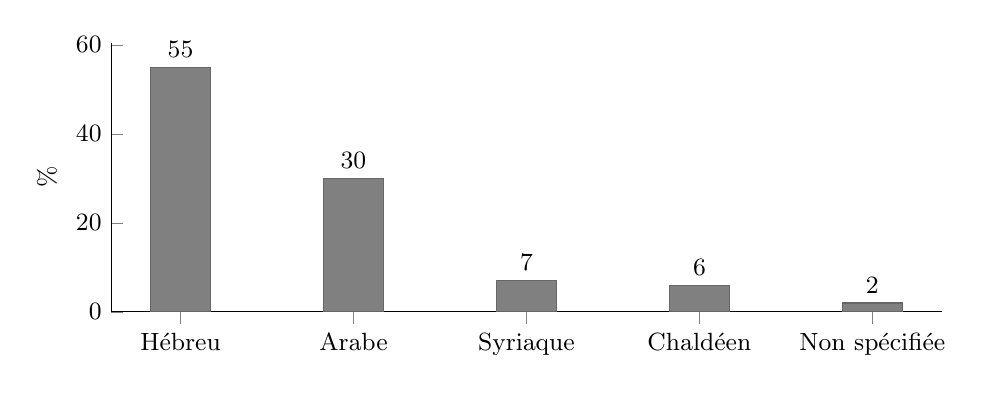
\begin{tikzpicture}
\begin{axis}
	[
	axis lines*=left,
	bar width=5ex,
	font=\small,
	height=5cm,
	nodes near coords,
	width=\textwidth,
	xtick=data,
	symbolic x coords={Hébreu,Arabe,Syriaque,Chaldéen,Non spécifiée},
	ybar=3pt,
	ylabel=\%,
	ylabel near ticks,
	ymin=0,
	]
	\addplot [fill=gray,draw=black!60]coordinates {(Hébreu,55) (Arabe,30) (Syriaque,7) (Chaldéen,6) (Non spécifiée,2)};
\end{axis}
\end{tikzpicture}
\caption{Distributions des langues -- lettre A}
\label{fig:kassi:1}
\end{figure}

\largerpage
Dans l’analyse du sous-corpus A on constate, quant à la distribution des langues (voir \figref{fig:kassi:1}), que 55~\% (102 attestations) concerne l’hébreu, 30~\% (56 attestations) l’arabe, 7~\% (12 attestations) le syriaque et 6~\% (11 attestations) le chaldéen. Le sous-corpus D représente une distribution similaire (62~\% pour l’hébreu, 21~\% pour l’arabe, 8~\% pour le chaldéen et 9~\% pour le syriaque).\clearpage

\begin{figure}
\begin{floatrow}
% % % \includegraphics[scale=1]{images/Kassiteridis_Figure2.png}
\ffigbox{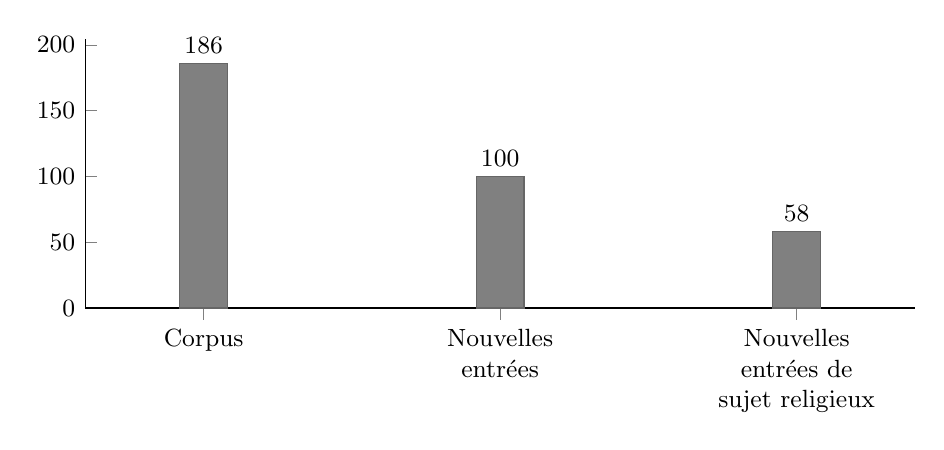
\begin{tikzpicture}
\begin{axis}
	[
	axis lines*=left,
	bar width=4ex,
	font=\small,
	height=5cm,
	nodes near coords,
	width=\linewidth,
	xtick=data,
	symbolic x coords={Corpus,Nouvelles entrées,Nouvelles entrées de sujet religieux},
	x tick label style={text width=2cm, align=center, font=\sloppy\small},
	ybar,
	ylabel near ticks,
	ymin=0,
	enlarge x limits=0.2
	]
	\addplot [fill=gray,draw=black!60]coordinates {(Corpus,186) (Nouvelles entrées,100) (Nouvelles entrées de sujet religieux,58)};
\end{axis}
\end{tikzpicture}}{\caption{Lettre A}\label{fig:kassi:2}}
\ffigbox{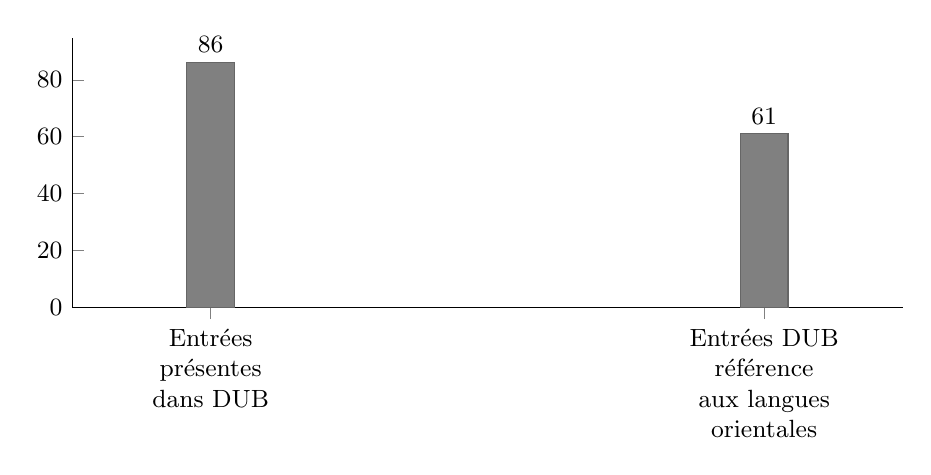
\begin{tikzpicture}
\begin{axis}
  [
	axis lines*=left,
	bar width=4ex,
	font=\small,
	height=5cm,
	nodes near coords,
	width=\linewidth,
	xtick=data,
	symbolic x coords={Entrées présentes dans DUB,Entrées DUB référence aux langues orientales},
	x tick label style={text width=2cm, align=center, font=\sloppy\small},
	ybar,
	ylabel near ticks,
	ymin=0,
	enlarge x limits=0.25
  ]
  \addplot [fill=gray,draw=black!60]coordinates {(Entrées présentes dans DUB,86) (Entrées DUB référence aux langues orientales,61)};
\end{axis}
\end{tikzpicture}}
{\caption{Entrées présentes dans le DUB\slash sans référence aux langues orientales}\label{fig:kassi:3}}
% % % \includegraphics[scale=1]{images/Kassiteridis_Figure3.png}
\end{floatrow}
\end{figure}

Passons à la comparaison entre le \emph{Dictionnaire universel de Trévoux} et celui de Basnage de Beauval~: dans le sous-corpus A, les 100 des 186 cas sont ajoutés par les rédacteurs du Trévoux, autrement dit, ils n’existent pas dans le dictionnaire de Basnage de Beauval (voir \figref{fig:kassi:2}). Parmi ces cas, plus de la moitié (58 cas) comporte un sujet religieux. Pour le sous-corpus D, une tendance similaire est constatée, notamment parmi les 63 entrées qui comprennent des langues orientales, les 41 sont de sujet religieux.

Néanmoins, les rédacteurs trévoltiens ne se limitent pas à ajouter de nouvelles entrées. Ils reformulent les entrées déjà présentes dans le \emph{Dictionnaire universel} de Basnage de Beauval (DUB dans la \figref{fig:kassi:3}) pour y inclure des références aux langues orientales. Comme représente la \figref{fig:kassi:3} ci-dessus, 46~\% des entrées du sous-corpus A (86 sur 186) existent déjà dans le dictionnaire de Basnage de Beauval et seulement 13~\% (25 sur 86) comprennent déjà des langues orientales.

\begin{figure}
% % % \includegraphics[scale=1]{images/Kassiteridis_Figure4.png}
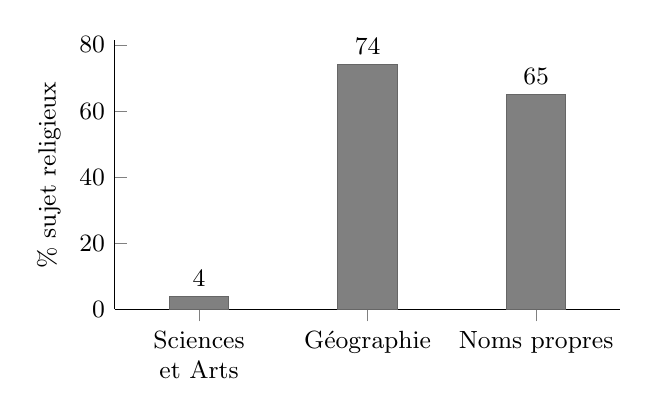
\begin{tikzpicture}
\begin{axis}
  [
	axis lines*=left,
	bar width=5ex,
	font=\small,
	height=5cm,
	nodes near coords,
	width=.66\textwidth,
	xtick=data,
	symbolic x coords={Sciences et Arts,Géographie,Noms propres},
	x tick label style={text width=2cm, align=center, font=\sloppy\small},
	enlarge x limits=0.25,
	ybar,
	ylabel near ticks,
	ymin=0,
	ylabel={\% sujet religieux}
  ]
  \addplot [fill=gray,draw=black!60]coordinates {(Sciences et Arts,4) (Géographie,74) (Noms propres,65)};
\end{axis}
\end{tikzpicture}
\caption{Proportion des sujets réligeux par thématique}
\label{fig:kassi:4}
\end{figure}

\begin{sloppypar}
À partir d’une analyse préliminaire des entrées qui comprennent ces langues, nous pouvons distinguer plusieurs domaines concernés tels que nom propre (\mbox{ABADDON}), géographie\footnote{Ce domaine n’existe en tant que tel dans le \emph{Dictionnaire universel de Trévoux} de 1721 et il regroupe les villes, villages, rivières, montages, lacs.} (ABARIM), grammaire (ACCENT), religion (ABÉLIENS), mythologie (ABADIR) mais aussi architecture (ABAQUE), botanique (ACACIA), médecine (ABDOMEN), monnaie (ABOKELLE). Cet éventail de sujets semble moins diversifié lorsque l’on approfondit les entrées permettant de trouver des références aux Écritures (57~\% du sous-corpus A et 63~\% du sous-corpus D est d’intérêt religieux, même s’il n'est pas toujours évident par le domaine indiqué). Par exemple, 65~\% des entrées du domaine «~noms propres~» et 74~\% des entrées géographiques dans le sous-corpus A présente un intérêt religieux. En revanche, cela ne se produit pas dans tous les domaines, puisque pour les entrées de sciences et d’arts ensemble, seule une sur 25 dans le sous-corpus A inclut un sujet religieux (voir \figref{fig:kassi:4}). Par ailleurs, 95~\% des entrées de noms propres et de géographie avec un sujet religieux sont ajoutés par le \emph{Dictionnaire universel de Trévoux}, puisque seules 2 (sur 38) existaient déjà dans le dictionnaire de Basnage de Beauval. Cette augmentation d’entrées sur les noms propres et la géographie ainsi que leur association aux sujets religieux nous amènent à penser que ces informations peuvent avoir un intérêt spécifique pour les rédacteurs du Trévoux. Dans le sous-corpus D, toutes les entrées de noms propres et 83~\% des entrées géographiques sont de sujet religieux. Il est donc possible que le texte dictionnairique soit conçu comme un guide ou un glossaire d’interprétation/traduction\footnote{On constate plusieurs références aux pratiques de traduction~: «~Cependant quelques nouveaux Critiques ont prétendu que dans une version Françoise de l'Ecriture on ne devoit se servir du mot d'adorer, que lorsqu'il étoit parlé du culte qui se rend à Dieu seul ~» dans ADORER~; «~ Il est mieux de traduire avec le Pere Amelotte, Abba, mon Pere~; ou plutôt avec M. Simon, Abba~; c’est-à-dire, mon Père~» dans ABBÉ.} de textes religieux, en désignant les villes, les rivières, les montagnes et les noms qui apparaissent aux Écritures. Richard Simon, considéré comme le principal rédacteur de la première édition du Trévoux 1704\footnote{Un avis soutenu aussi par les \emph{Mémoires} de Nicéron et le supplément au \emph{Grand dictionnaire historique} de Moréri, \citet[598]{Graveleau2018}.}, dans son œuvre \emph{Histoire critique du Vieux Testament}, invite dans une nouvelle traduction de l’Ancien Testament «~à joindre un dictionnaire de la langue hébraïque, mais aussi des outils d’histoire, comme un dictionnaire généalogique, un autre géographique, etc. ~» \citep{Laplanche1994}, ce qui nous semble coïncider avec les additions d’intérêt exégétique dans le Trévoux. L’exégète dieppois a même remarqué dans sa lettre XXV \citep[220--226]{Simon1730} un tel dictionnaire, à savoir le \emph{Dictionnaire hébreu-italien des mots difficiles de la Bible} (1612) de Léon de Modène (1571--1648), un dictionnaire dont les Juifs «~ se servent pour apprendre aux enfans à expliquer le Texte Hebreu de la Bible~» soulignant l’utilité d’un tel ouvrage pour bien traduire l’Écriture Sainte.
\end{sloppypar}

L’importance des noms propres a également été soulignée par nos rédacteurs dans la Préface du dictionnaire~: 
\begin{quote}
    les noms propres n’ont-ils pas leurs significations, leur étymologie, leur orthographe, leurs variations, leurs nombres, leur usage \& leurs difficultez, comme tous les autres~? […] Ne doit-on pas sçavoir comment il faut les traduire des autres Langues, \& les exprimer dans la nôtre~? […] Qu’on écrive l’Histoire, sur-tout Ecclésiastique, ou la Vie des Saints, sans être instruit de la manière dont nous avons travesti les noms propres dans notre Langue […] Combien de ces sortes de mots, qui dans leur origine étant les mêmes, ont néanmoins dans notre Langue presque autant de différentes formes, qu'il y a de différens Saints qui les ont eus, ou de différens lieux, où le culte de ces Saints s'est établi~? Quelle confusion l'ignorance de l'usage ne produira-t-elle pas.
\end{quote} 
Cet intérêt pour les noms propres n’est pas nouveau. Comme le signale Richard Simon dans une autre lettre («~Lettre XXXV~» dans \citealt[286--294]{Simon1730}), Robert Estienne (1503--1559) a également rédigé des ouvrages consacrés (i) aux catalogues de noms propres, de villes, de montagnes, etc.\footnote{\emph{Voir Dictionarium propriorum nominum virorum, mulierum, populorum, idolorum, urbium, fluviorum, montium caeterorumque locorum quae passim in libris prophanis leguntur} (1541).}, (ii) à la manière dont il faut traduire des noms propres de latin en français\footnote{Voir \emph{La maniere de tourner toutes especes de noms latins en nostre langue françoyse. Reveue et corrigée soigneusement à l’utilité des jeunes enfants} (1546).} (iii) ainsi qu’aux noms hébreux, chaldéens, grecs, latins attestés dans la Bible et leurs interprétations\footnote{Voir \emph{Hebraea, chaldaea, graeca et latina nomina quae in Bibliis leguntur, restituta, cum latina interpretatione. Locorum descriptio ex cosmographi} (1537).}, ce qui résonne avec la pratique constatée dans le \emph{Dictionnaire universel de Trévoux}. Ces éléments nous amènent à considérer qu’il s’agit alors d’un dictionnaire-guide écrit pour reprendre l’autorité d’interprétation (en passant par la traduction) des Écritures, contestée par les huguenots.  

Cette autorité tente d’être rétablie par l’expertise en langues orientales, outil indispensable pour «~un bon Interprète de l’Ecriture~» (dans HÉBREU). Dans ce cadre, l’hébreu sert souvent de langue-source d’un mot (étymologie) ou d’élément d’association entre langues (équivalent). Le statut de l’hébreu comme langue de l’Ancien Testament et comme «~la plus ancienne langue qu’il ait eue au monde ~» (dans HÉBREU), ainsi que l’utilité de l’étymologie pour «~comprend mieux la force \& la signification des mots~»\footnote{Voir «~aussi car pour expliquer les termes plus précisément, il faut retourner à la première imposition, afin de parler juste, \& de bien entendre ce que l’on dit  ~» dans ÉTYMOLOGIE.} (dans ÉTYMOLOGIE) peuvent justifier la mise en application de la langue hébraïque comme ressource étymologique d’autorité visant à figer une interprétation précise des éléments de l’Écriture. Néanmoins, l’hébreu ne peut pas établir à lui seul une interprétation exacte, puisque dans l’Ancien Testament «~il y a même quelques parties qui sont en Chaldaïque, \& differens mots Chaldaïques, ou de quelques autres langues, répandus en différens endroits ~» (dans HÉBREU). En outre, l'hébreu étant une langue source assez obscure (interprétation liée à la verbalisation différente des radicaux ou des consonnes subissant des substitutions lors de la copie), a amené les critiques à s’intéresser à la comparaison des versions existantes\footnote{On peut tracer l’intérêt sur les relations entre des langues sémitiques au XVIe siècle dans les travaux de Joseph-Juste Scaliger et Isaac Casaubon \citep{Laplanche1994}} afin de reconstituer «~le sens véritable~». Ainsi, nous trouvons dans le Trévoux des langues considérées comme des dialectes de l’hébreu\footnote{«~Les langues Chaldaïque, Syriaque, Ethiopienne, Arabe, \&c. sont des dialectes de l’Hébreu, comme les langues Françoise, Italienne, Espagnole, Portugaise, sont des dialectes du Latin ~», dans HÉBREU.}, langues aussi pertinentes pour les versions traduites de l’Ancien Testament, dont la présence a un objectif similaire à celui de l’hébreu. Ceci est illustré par la comparaison de différents équivalents\footnote{À titre d’exemple, «~Au reste, quoique le texte Hebreu porte אבנח , Abana, aussi-bien que la Vulgate, cependant le Keri, ou Variante, porte אמנח , Amana, \& les Septante l'ont ainsi écrit, 'Αμανὰ ~», dans ABANA.},  pratique associée à la méthode historico-critique de la Bible liée à l'œuvre de Richard Simon. 

Je pense qu’il vaut mieux s’arrêter un instant sur la pensée de ce savant, pour clarifier l’enjeu du dictionnaire. Richard Simon dans son ouvrage \emph{Histoire critique des principaux commentateurs du Nouveau Testament} (1693) a mis en question la validité de l’interprétation biblique de St. Augustin sur laquelle se fonde la tradition catholique \citep[255]{Tambrun2020}. L’interprétation augustinienne - selon Richard Simon dans les \emph{Additions aux «~Recherches curieuses sur la diversité des langues et religions~» d’Edward Brerewood} (1677) - dérivait de la tradition antérieure en raison de son ignorance de l’hébreu et du grec \citep[261]{Le-brun2012}. Ainsi, Richard Simon a tenté, à partir de la comparaison des sources, d’atteindre le sens de l’Écriture avant cette dérivation interprétative \citet[256]{Tambrun2020}. Afin d’être plus précis dans l’interprétation biblique, la connaissance des langues hébraïque et grecque est indispensable pour le recours aux textes originaux et leur comparaison avec la Vulgate \citep[6]{Simon1730}. Ceci s’appuie sur la nécessité d’une, disons, professionnalisation de l’exégèse, «~le seul Art dont tout le monde se meste  ~» \citep[3]{Simon1730}.  Richard Simon se garde bien de renoncer à l'autorité de la Vulgate établie par le Concile de Trente (en 1551--1552 et en 1562--1563), mais il soutient que la méthode comparative permet de mieux la comprendre \citet[4]{Simon1730}. Cette méthode sert également d’outil de prosélytisme pour les huguenots en démontrant la similitude de la Vulgate, dont ceux-ci ne reconnaissent pas l'autorité, avec les autres versions \citep[5]{Simon1730}.

Cet intérêt pour les langues sémitiques s’inscrit dans ce contexte et se manifeste également dans les entrées grammaticales (A, ACCENT) où les rédacteurs nous aident à comprendre les spécificités de ces langues et leurs différences avec le français\footnote{«~C’est inutilement que la plûpart des Grammairiens comparent la Lettre a des Latins \& des François, avec l’aleph des Hébreux \& l’eliph des Arabes~; parceque ces deux Lettres n’ont aucun rapport avec notre a, si ce n’est qu’elles sont les premières dans l’Alphabet Hébreu \& dans celui des Arabes~; mais elles ne sont pas des voyelles comme dans la Langue Françoise ~», dans A.} tout en montrant leur expertise qui justifie leur capacité à corriger d’autres auteurs. Par exemple, à l’entrée AIN, lettre hébraïque et arabe, son absence dans les langues européennes est soulignée «~Nous n’avons point […] dans nos langues d’Europe~»~; les rédacteurs du Trévoux tentent de mettre cette entrée en relation avec les différentes méthodes de traduction/translittération des mots hébreux contenant la lettre ain «~ע~»  en grec («~les Septante ont rendu cette lettre de deux manières différentes tantôt sans aspiration, comme dans עדן qu’ils expriment Ἐδὲν, Eden~; \& tantôt par un Γ, c’est-à-dire un G, comme dans עמורה qu’ils traduisent Γόμοῤῥα, Gomorrha~») et en latin «~ (Quelques Grammairiens qui l’expriment par ng, d’autres par gn~»).

Reprenons maintenant les noms propres qui servent non seulement de glossaire pour l’interprétation et la traduction des Écritures, comme mentionné ci-dessus, mais aussi de scène pour démontrer et valoriser la méthode étymologique et comparative~; pour les rédacteurs trévoltiens, «~c'est principalement par la connoissance des noms propres, que l'on apprend bien les origines, \& les principes d'une Langue, \& que l'on se rend habile dans la science des étymologies ~» (Préface) - un élément essentiel pour leur interprétation des éléments religieux. Selon \citet{Thebaud-sorger2015}, la mise en scène d’objets et de phénomènes scientifiques, comme les démonstrations publiques d’expériences d’électricité de l’abbé Nollet ou l’expérience de Rouen de Blaise Pascal sur l’existence du vide, peut être considérée comme constitutive de la science moderne. Le public de la cour, puis des salons et des sociétés savantes, a privilégié ce «~théâtre de la preuve~». Dans le contexte d’un dictionnaire adressé à un grand public, il faut prendre en compte la valeur de ce spectacle textuel (d’une méthode qui tente de s’établir comme autoritaire) comme outil de valorisation et de vulgarisation. Pour illustrer cette démonstration, examinons l’analyse étymologique méticuleusement menée par les rédacteurs du \emph{Dictionnaire universel de Trévoux} dans l’entrée ARAIGNÉE~: ils commencent par présenter l’hypothèse erronée que quelques-uns, comme Basnage de Beauval dans son dictionnaire, soutiennent selon laquelle ce mot vient du grec «~ἀράχνη~» ou même «~ἀραιὸς~». Ils présentent ensuite leur propre hypothèse qui est «~bien plus vraisemblable ~» en recherchant les origines de ce mot dans le mot hébreu «~ארג~» qui signifie «~faire un tissu~». Ils mettent en évidence les explications erronées liées à l’hypothèse hébraïque (comme celle dans le dictionnaire de Moréri qui a soutenu que «~arag~» [ארג] signifie araignée en hébreu) et ils soutiennent la leur, à savoir que «~arag~» signifie faire de la toile, en se référant à l'utilisation de ce mot hébreu chez David de Pomis ainsi que chez un autre rabbin appelé Menahhem. Enfin, ils démontrent en détail les changements phonétiques qui aboutissent du mot hébreu «~arag~» au mot grec «~ἀράχνη~», puis au latin «~aranea~» («~ le G Hébreu s’est changé en Grec χ, de même que souvent le χ Grec se change en G Latin~») en soulignant la régularité de ces changements phonétiques par référence à d’autres mots («~comme en χαλβάνη, Galbanum~; λείχω, lingo~; ἀΓχω, ango~»), ainsi que par référence à d’autres Grammairiens (Hieroz, P. Thomassin).  Ils présentent ainsi leur méthode étymologique qui se fonde sur la régularité des correspondances linguistiques, l’usage ainsi que les travaux d’autres membres de la communauté savante et non sur l’assemblage non critique des idées d’autres auteurs. L’emploi de ces langues dans des entrées sans intérêt religieux comme la Botanique, l’Architecture, la Médecine peut être justifié à la lumière de la mise en scène de la méthode d’interprétation des rédacteurs~; or, une autre interprétation est possible puisque les rédacteurs trévoltiens reconnaissent dans la Préface et dans certaines entrées, l’impact des peuples sémitiques sur les connaissances scientifiques (voir ASTRONOMIE)~; leur présence dans des entrées de domaines scientifiques peut aussi être liée à cela. Les entrées pertinentes de la lettre A et D ne témoignent cependant pas d'une telle interprétation, car il n'y a rien sur l'importance des travaux des peuples sémites en médecine, en botanique ou en architecture.

Ce que semble viser la présence des langues orientales dans le \emph{Dictionnaire universel de Trévoux}, c'est d’offrir un guide de lecture (et par conséquent d’interprétation et de traduction) des textes religieux de façon à valoriser leur méthode philologique. Par conséquent, ce guide sert d’outil de prosélytisme par la reconstitution d’une interprétation «~exacte~» des Écritures. L’hébreu, l’arabe, le syriaque, le chaldéen étant des langues étroitement associées à l’histoire des Écritures, elles deviennent stratégiques dans le contexte de la méthode exégétique historico-critique. Contrairement aux langues européennes, les langues orientales n’appartiennent pas à la même famille que le français, ces sont des reliques obscures et l’intérêt qu’on leur porte est principalement de nature érudite. Cependant, on constate un intérêt ethnographique par le biais de l’histoire comparée des religions et des entrées du domaine «~Relations~» qui nécessite une étude plus approfondie.


\appendixsection{Les caractéristiques des «~langues orientales~» selon le \emph{Dictionnaire universel de Trévoux} (1721), Lettre A.}

\begin{description}[font=\normalfont]
\item[ACHAL] 
    \begin{itemize}[leftmargin=*]
        \item[]
        \item Extrait: Le mot achal dans les langues orientales signifie tuer \& manger. 
        \item Caractéristique linguistique: Existence du mot «~achal~» avec la signification \emph{tuer} \& \emph{manger}.
    \end{itemize}        
\item[ABYSSINS] 
    \begin{itemize}[leftmargin=*]
        \item[]
        \item Extrait: Cette langue [le caldéenne] a des caracteres particulieurs, \& elle n’a pas des points voyalles separez des consones, comme il y en a dans l’Hebreu \& dans les autres langues Orientales. 
        \item Caractéristique linguistique: Langues écrites en abjad. Le caldéen et l’hébreu appartiennent aux langues orientales.
    \end{itemize}        
\item[AIN] 
    \begin{itemize}[leftmargin=*]
        \item[]
        \item Extrait: C’est le nom d’une lettre, qui est une aspiration passée par le nez. Toutes les langues orientales ont le ain. 
        \item Caractéristique linguistique: Lettre aspirée «~ain~». 
    \end{itemize}        
\item[ASPIRATION]
    \begin{itemize}[leftmargin=*]
        \item[]
        \item Extrait: Une seconde raison que ce sont des consones, c’est que les langues Orientales qui n’expirmoient point les voyelles, ont cependant toûjours éxprimé les aspirations. 
        \item Caractéristique linguistique: Lettres aspirées. Langues qui n’expriment pas de voyelles. 
    \end{itemize}
\newpage
\item[AUGMENT] 
    \begin{itemize}[leftmargin=*]
       \item[]
        \item Extrait: Ce tèrme d’augment syllabique, qui n’est en usage que lorsqu’on parle de la langue Grécque, pourroit être appliqué à la Grammaire des langues Orientales, où la même chose arrive. 
       \item Caractéristique linguistique: Augment syllabique. Grec n’appartient pas aux langues orientales. 
    \end{itemize}       
\end{description}

{\sloppy\printbibliography[heading=subbibliography,notkeyword=this]}
\end{otherlanguage}
\end{document}
